\documentclass[twocolumn]{aastex631}
\bibliographystyle{aasjournal}

\usepackage{graphicx}
\usepackage[caption=false]{subfig}
\usepackage{amsmath}
\usepackage{booktabs}
\usepackage{censor}

\let\pwiflocal=\iffalse \let\pwifjournal=\iffalse
%From: http://arxiv.org/format/1512.00483
%\input{setup}
%\input{mgs_setup}

%% General
\newcommand{\msini}{\ensuremath{m \sin i}}
\newcommand{\mplsini}{\ensuremath{\mpl\sin i}}
\newcommand{\teff}{\ensuremath{T_{\rm eff}}}
\newcommand{\logg}{\ensuremath{\log{g}}}
\newcommand{\vsini}{\ensuremath{v \sin{I_\star}}}
\newcommand{\feh}{\ensuremath{\rm [Fe/H]}}
\newcommand{\logl}{\ensuremath{\log{L}}}
\newcommand{\vmac}{\ensuremath{v_{\rm mac}}}
\newcommand{\vmic}{\ensuremath{v_{\rm mic}}}
% Activity index R'_HK
\newcommand{\rhk}{\ensuremath{R^{\prime}_{HK}}}
% log of R'_HK
\newcommand{\logrhk}{\ensuremath{\log\rhk}}
% S average value
\newcommand{\Savg}{\ensuremath{\langle S\rangle}}


%% ---------------------------------------------------------------------
%% Solar quantities 
\newcommand{\rsun}{\ensuremath{R_\sun}}
\newcommand{\msun}{\ensuremath{M_\sun}}
\newcommand{\lsun}{\ensuremath{L_\sun}}
\newcommand{\loglsun}{\ensuremath{\log{L_\sun}}}
\newcommand{\teffsun}{\ensuremath{T_{eff,\sun}}}
\newcommand{\rhosun}{\ensuremath{\rho_\sun}}
\newcommand{\loggsun}{\ensuremath{\log{g_{\sun}}}}

%% ---------------------------------------------------------------------
%% Stellar quantities 
\newcommand{\rstar}{\ensuremath{R_\star}}
\newcommand{\mstar}{\ensuremath{M_\star}}
\newcommand{\lstar}{\ensuremath{L_\star}}
\newcommand{\astar}{\ensuremath{a_\star}}
\newcommand{\loglstar}{\ensuremath{\log{L_\star}}}
\newcommand{\teffstar}{\ensuremath{T_{\rm eff\star}}}
\newcommand{\rhostar}{\ensuremath{\rho_\star}}
\newcommand{\loggstar}{\ensuremath{\log{g_{\star}}}}

%% ---------------------------------------------------------------------
%% Earth
\newcommand{\rearth}{\ensuremath{R_\earth}}
\newcommand{\mearth}{\ensuremath{M_\earth}}
\newcommand{\learth}{\ensuremath{L_\earth}}
\newcommand{\teffearth}{\ensuremath{T_{\rm eff,\earth}}}
\newcommand{\rhoearth}{\ensuremath{\rho_\earth}}

%% ---------------------------------------------------------------------
%% Planetary
\newcommand{\rpl}{\ensuremath{R_{p}}}
\newcommand{\mpl}{\ensuremath{M_{p}}}
\newcommand{\lpl}{\ensuremath{L_{p}}}
\newcommand{\teffpl}{\ensuremath{T_{\rm eff,{p}}}}
\newcommand{\rhopl}{\ensuremath{\rho_{p}}}
\newcommand{\ipl}{\ensuremath{i_{p}}}
\newcommand{\epl}{\ensuremath{e_{p}}}
\newcommand{\gpl}{\ensuremath{g_{p}}}
\newcommand{\loggpl}{\ensuremath{\log g_{p}}}

\newcommand{\arstar}{\ensuremath{a/\rstar}}
\newcommand{\zrstar}{\ensuremath{\zeta/\rstar}}

%% ---------------------------------------------------------------------
%% Jupiter
\newcommand{\rjup}{\ensuremath{R_{\rm J}}}
\newcommand{\mjup}{\ensuremath{M_{\rm J}}}
\newcommand{\ljup}{\ensuremath{L_{\rm J}}}
\newcommand{\teffjup}{\ensuremath{T_{eff,{\rm J}}}}
\newcommand{\rhojup}{\ensuremath{\rho_{\rm J}}}
\newcommand{\gjup}{\ensuremath{\g_{\rm J}}}

\newcommand{\rjuplong}{\ensuremath{R_{\rm Jup}}}
\newcommand{\mjuplong}{\ensuremath{M_{\rm Jup}}}
\newcommand{\ljuplong}{\ensuremath{L_{\rm Jup}}}
\newcommand{\teffjuplong}{\ensuremath{T_{eff,{\rm Jup}}}}
\newcommand{\rhojuplong}{\ensuremath{\rho_{\rm Jup}}}
\newcommand{\gjuplong}{\ensuremath{\g_{\rm Jup}}}

\providecommand{\eprint}[1]{\href{http://arxiv.org/abs/#1}{#1}}
\providecommand{\adsurl}[1]{\href{#1}{ADS}}
\newcommand{\project}[1]{\textsl{#1}}

\begin{document}
\shorttitle{HPF spectral analysis}
\shortauthors{TBD}

\title{Atmospheric escape and star-planet-interaction in the HAT-P-67 b system}

\author{TBD}
\affiliation{TBD}


\begin{abstract}
    We aim to understand how exoplanet atmospheres evolve across age, stellar irradiation environments, planet properties, and---for extremely close-in exoplanets---direct star-planet interaction (SPI) such as stellar winds, tidal forces, and magnetic interactions. The scarcity of exoplanet atmosphere measurements across a range of stellar properties has limited our ability to complete this picture.

    The Helium Exospheres program with the Habitable Zone Planet Finder (HPF) spectrograph on the Hobby Eberly Telescope (HET) in West Texas has targeted 23 exoplanet systems over two years. Here, we present a study of HAT-P-67, an F subgiant hosting a low density planet with 0.3 $M_{\mathrm{Jup}}$ and 2.1 $R_{\mathrm{Jup}}$ on a close-in 4.8 day orbit. The high energy radiation environment should provide a uniquely harsh testing ground for examining atmospheric escape. The planet shows prominent in-transit absorption in the He 10830 \AA~ triplet and infrared Ca II 8542 \AA~ triplet across 20 visits over the course of a year including in- and out-of-transit spectroscopy. We identify the rotational period of HAT-P-67 to be 5.417 days by using contemporaneous data from the Transiting Exoplanet Survey Satellite (TESS). We consider multiple interpretations of the HPF and TESS observations. First, the period measured by TESS may be the rotational period of the star and thus, the star and planet are nearly-tidally locked. On the other hand, the period measured by TESS may result from SPI-induced hot spots on the surface that follow the magnetic field lines linked to the planet's orbital period. Finally, we consider the possibility of stellar surface inhomogeneity contaminating the He and Ca II transit signals.
\end{abstract}

\keywords{stars: fundamental parameters ---  stars: statistics}

\section{Introduction}\label{sec:intro}

Exoplanets possess a dynamic range of atmospheric properties far beyond what we have seen in our own Solar System.  Extreme radiation effects, atmospheric erosion, and unexpected chemistry must exist, but collecting examples of these phenomena remains at the edge of the possible today. The minuscule signal strengths of atmospheric shells has hidden all but the most conspicuous phenomena.  Helium 10830 \AA has emerged as the most conspicuous exosphere indicator, enabling ground-based detection with high-resolution near-infrared (IR) spectrographs.

At least 8 systems have Helium 10830 exosphere measurements to date: \object[GJ 3470]{GJ3470} \citep{2020ApJ...894...97N, 2021A&A...647A.129L}, \object{HD 63433 c} \citep{2022AJ....163...68Z}, WASP 107 b \citep{2019A&A...623A..58A,2020AJ....159..115K}, HD 209458 b \citep{2019A&A...629A.110A}, WASP 69 b \citep{2020AJ....159..278V}, WASP 52 b \citep{2020AJ....159..278V}, HD 189733 b \citep{2021A&A...647A.129L}, and HAT-P-18 b \citep{2021ApJ...909L..10P}.


Here we present a study of the exosphere of HAT-P-67b.  HAT-P-67 is an F type sub-giant with the Saturn-sized planet HAT-P-67b.  HAT-P-67b stands out for a few reasons.  It has a relatively low surface gravity, which could make it amenable to rapid atmospheric mass loss.  It orbits an evolved star, which means its instellation may have increased as the star's size has grown.  The star appears close to the star, making it conceivable that star-planet interactions could be at play.  These and other reasons make HAT-P-67b a unique laboratory for measuring the properties of exospheres and their interactions with their host stars.  The system appears to consist of a binary with an M dwarf companion HAT-P-67B separated by $9\farcs0$.

\section{Observations}
\subsection{Habitable Zone Planet Finder (HPF)}

The Habitable Zone Planet Finder Spectrograph \citep[HPF][]{2012SPIE.8446E..1SM,2014SPIE.9147E..1GM, 2019Optic...6..233M} on the queue-scheduled 10-meter \emph{Hobby-Eberly Telescope} \citep[HET][]{1998SPIE.3352...34R, 2007PASP..119..556S} operates in the near-IR from $8100-12800~\AA\;$ spanning the \textit{z}, \textit{Y}, and \textit{J} bands. We observed HAT-P-67b with HPF in-transit on 2020 April 28, 2020 May 22, and 2020 June 15 and out-of-transit on a total of \censorbox{xx} other nights.


\begin{deluxetable}{lcc}
    \tablecaption{HPF Observations for HAT-P-67b \label{tab:observation_properties}}
    \tablehead{
        \colhead{Date} & \colhead{Time of Observation} & \colhead{Transit}}
    \startdata
    2020-04-28 & 06:10:31 & In transit\\
    2020-04-28 & 06:16:12 & In transit\\
    2020-04-28 & 06:21:53 & In transit\\
    2020-04-28 & 06:27:34 & In transit\\
    2020-04-28 & 06:33:15 & In transit\\
    2020-04-28 & 06:38:57 & In transit\\
    2020-04-28 & 06:44:38 & In transit\\
    2020-04-28 & 06:50:19 & In transit\\
    \enddata
\end{deluxetable}

\subsection{TESS Light Curve}
HAT-P-67 was observed with the \emph{Transiting Exoplanet Survey Satellite} \citep[TESS][]{2014SPIE.9143E..20R} in Sectors 24, 26, 51, 52, 53 with 2-minute cadence, and in Sector 25 with 30-minute (FFI) cadence.  The Sector 25 FFI data appeared malformed, possibly due to problems with pipeline CCD smear correction, and was disregarded.

\subsection{ASAS-SN}
We retrieved ground-based photometry with the \emph{All-Sky Automated Survey for Supernovae} (ASAS-SN) using the Sky-Portal \citep{shappee14,2017PASP..129j4502K}.

\subsection{DASCH}
We searched for observations of HAT-P-67 in other archives.  It appears in the Harvard Plate Archive, with 5809 measurements digitized through DASCH \censorbox{citation}, spanning over 120 years of coarse photometric monitoring.  In principle these datasets could inform long-term variability trends such as stellar cycles.  In practice the 0.15 magnitude jitter appears too coarse to perceive any genuine astrophysical variability, with no conspicuous trend seen.  We can therefore place a relatively mild constraint that the star is stable at the $30\%$ level over periods of tens of years.

\subsection{Gaia DR3}
HAT-P-67A (\emph{Gaia DR3 1358614983131339392}) has a parallax of $2.69\pm0.01$ mas in \emph{Gaia} DR3, placing it at about 372$\pm$1.4 pc, slightly farther than previously estimated by \citet{2017AJ....153..211Z} using Gaia DR1. Its coarse Gaia-based estimates for RV and Doppler broadening are consistent with the more precise values published in \citet{2017AJ....153..211Z}.  Its wide companion HAT-P-67B (\emph{Gaia DR3 1358614983131339904}) \citep{2019MNRAS.490.5088M} has statistically identical parallax ($2.58\pm0.05$) and proper motions, confirming its interpretation as co-moving, with projected separation of about 3400 AU.

\subsection{Other archives}
We searched for observations of HAT-P-67 in public archives.  It has one $R\sim8000$ spectrum from the Intermediate Dispersion Spectrograph on the INT, centered near 4000 $\AA$.  It has 26 photometry points from \emph{Pan-STARRS} spread across its 5 filters.  The other archival observations have been previously reported by \citet{2017AJ....153..211Z}, including Keck HIRES, Keck NIRC2, and WIYN High-Resolution Infrared Camera.  The northern source does not appear in ESO archives, nor the Gemini Archive, and it is not publicly accessible in the Zwicky Transient Factory (ZTF) archive.  It was not targeted by Spitzer or Hubble.



\section{Analysis}

\begin{figure}
    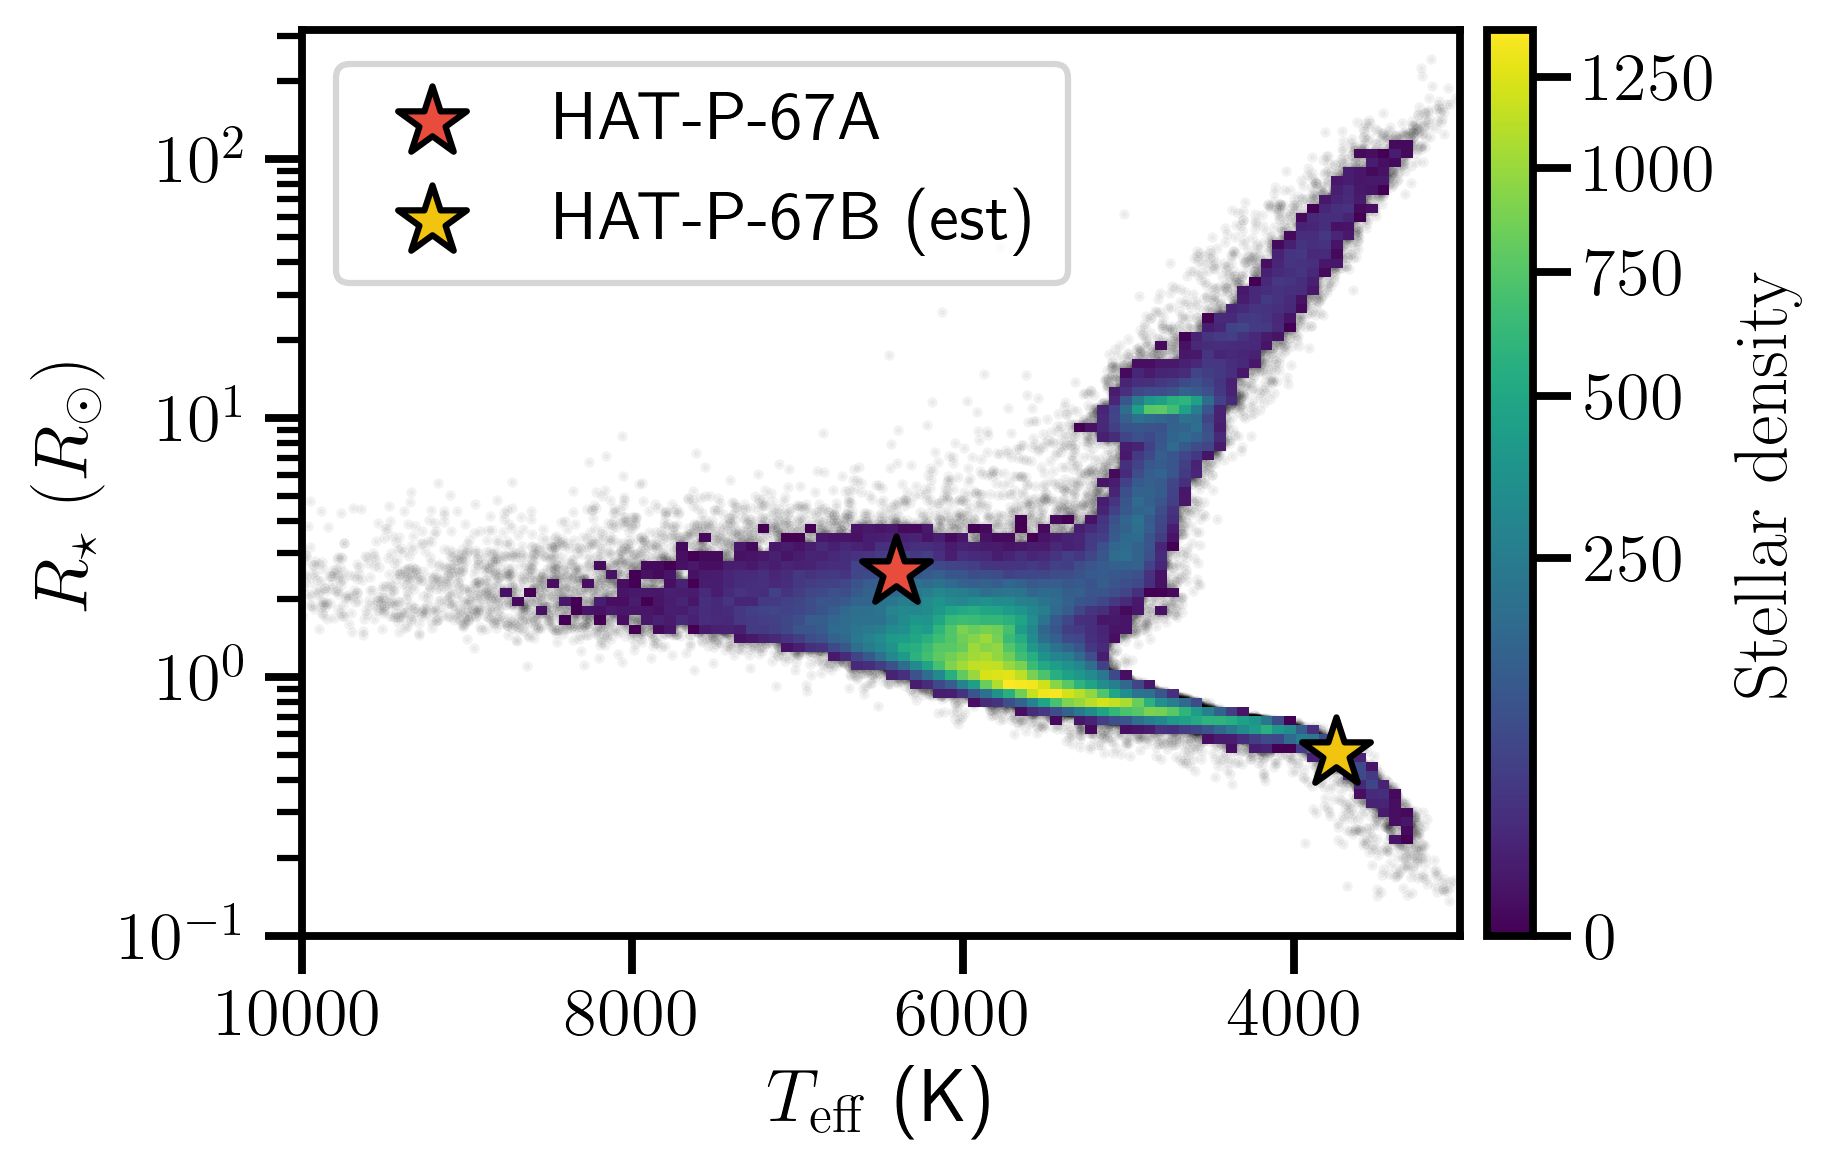
\includegraphics[width=\linewidth]{figures/Gaia_HAT_P_67_AB.png}
    \caption{HR Diagram of F star HAT-P-67A with its assumed M-dwarf main sequence companion HAT-P-67B.  The density of stars comes from the \emph{Kepler} prime field estimated by \citet{2020AJ....160..108B} using \emph{Gaia DR2}.}
    \label{fig:gaiaHRD}
\end{figure}


\subsection{TESS Light Curve}

\subsubsection{Revised exoplanet orbital parameters}
We assembled a composite lightcurve by stitching TESS Sectors 24, 26, 51, 52, 53, which were reduced with the default SPOC pipeline \citep{2020RNAAS...4..201C}, and lightly post-processed with \texttt{lightkurve} \citep{geert_barentsen_2019_2565212}.  These TESS data exhibit an RMS scatter of better than 1 part-per-thousand (ppt) at native 2-minute sampling.  We fit a Keplerian orbit model to the TESS lightcurve using the \texttt{exoplanet} framework \citep{exoplanet:joss}.  We obtained a best fit orbital period of $4.81011$ days, non-zero eccentricity of 0.19, an impact parameter of 0.46, planet-to-star radius of 0.0823, transit depth of 0.74\%, and $T_0$ of 1958.07933 in BTJD.  We did not attempt MCMC sampling to quantify degeneracy among these parameters, and we suspect that the transit is adequately modeled by a circular orbit.  Figure \ref{fig:transit} shows the best-fit orbit overlaid on the detrended TESS lightcurve.  Table \ref{tabOrbit} lists a previous orbit determination and solutions reported here.


\begin{figure}
    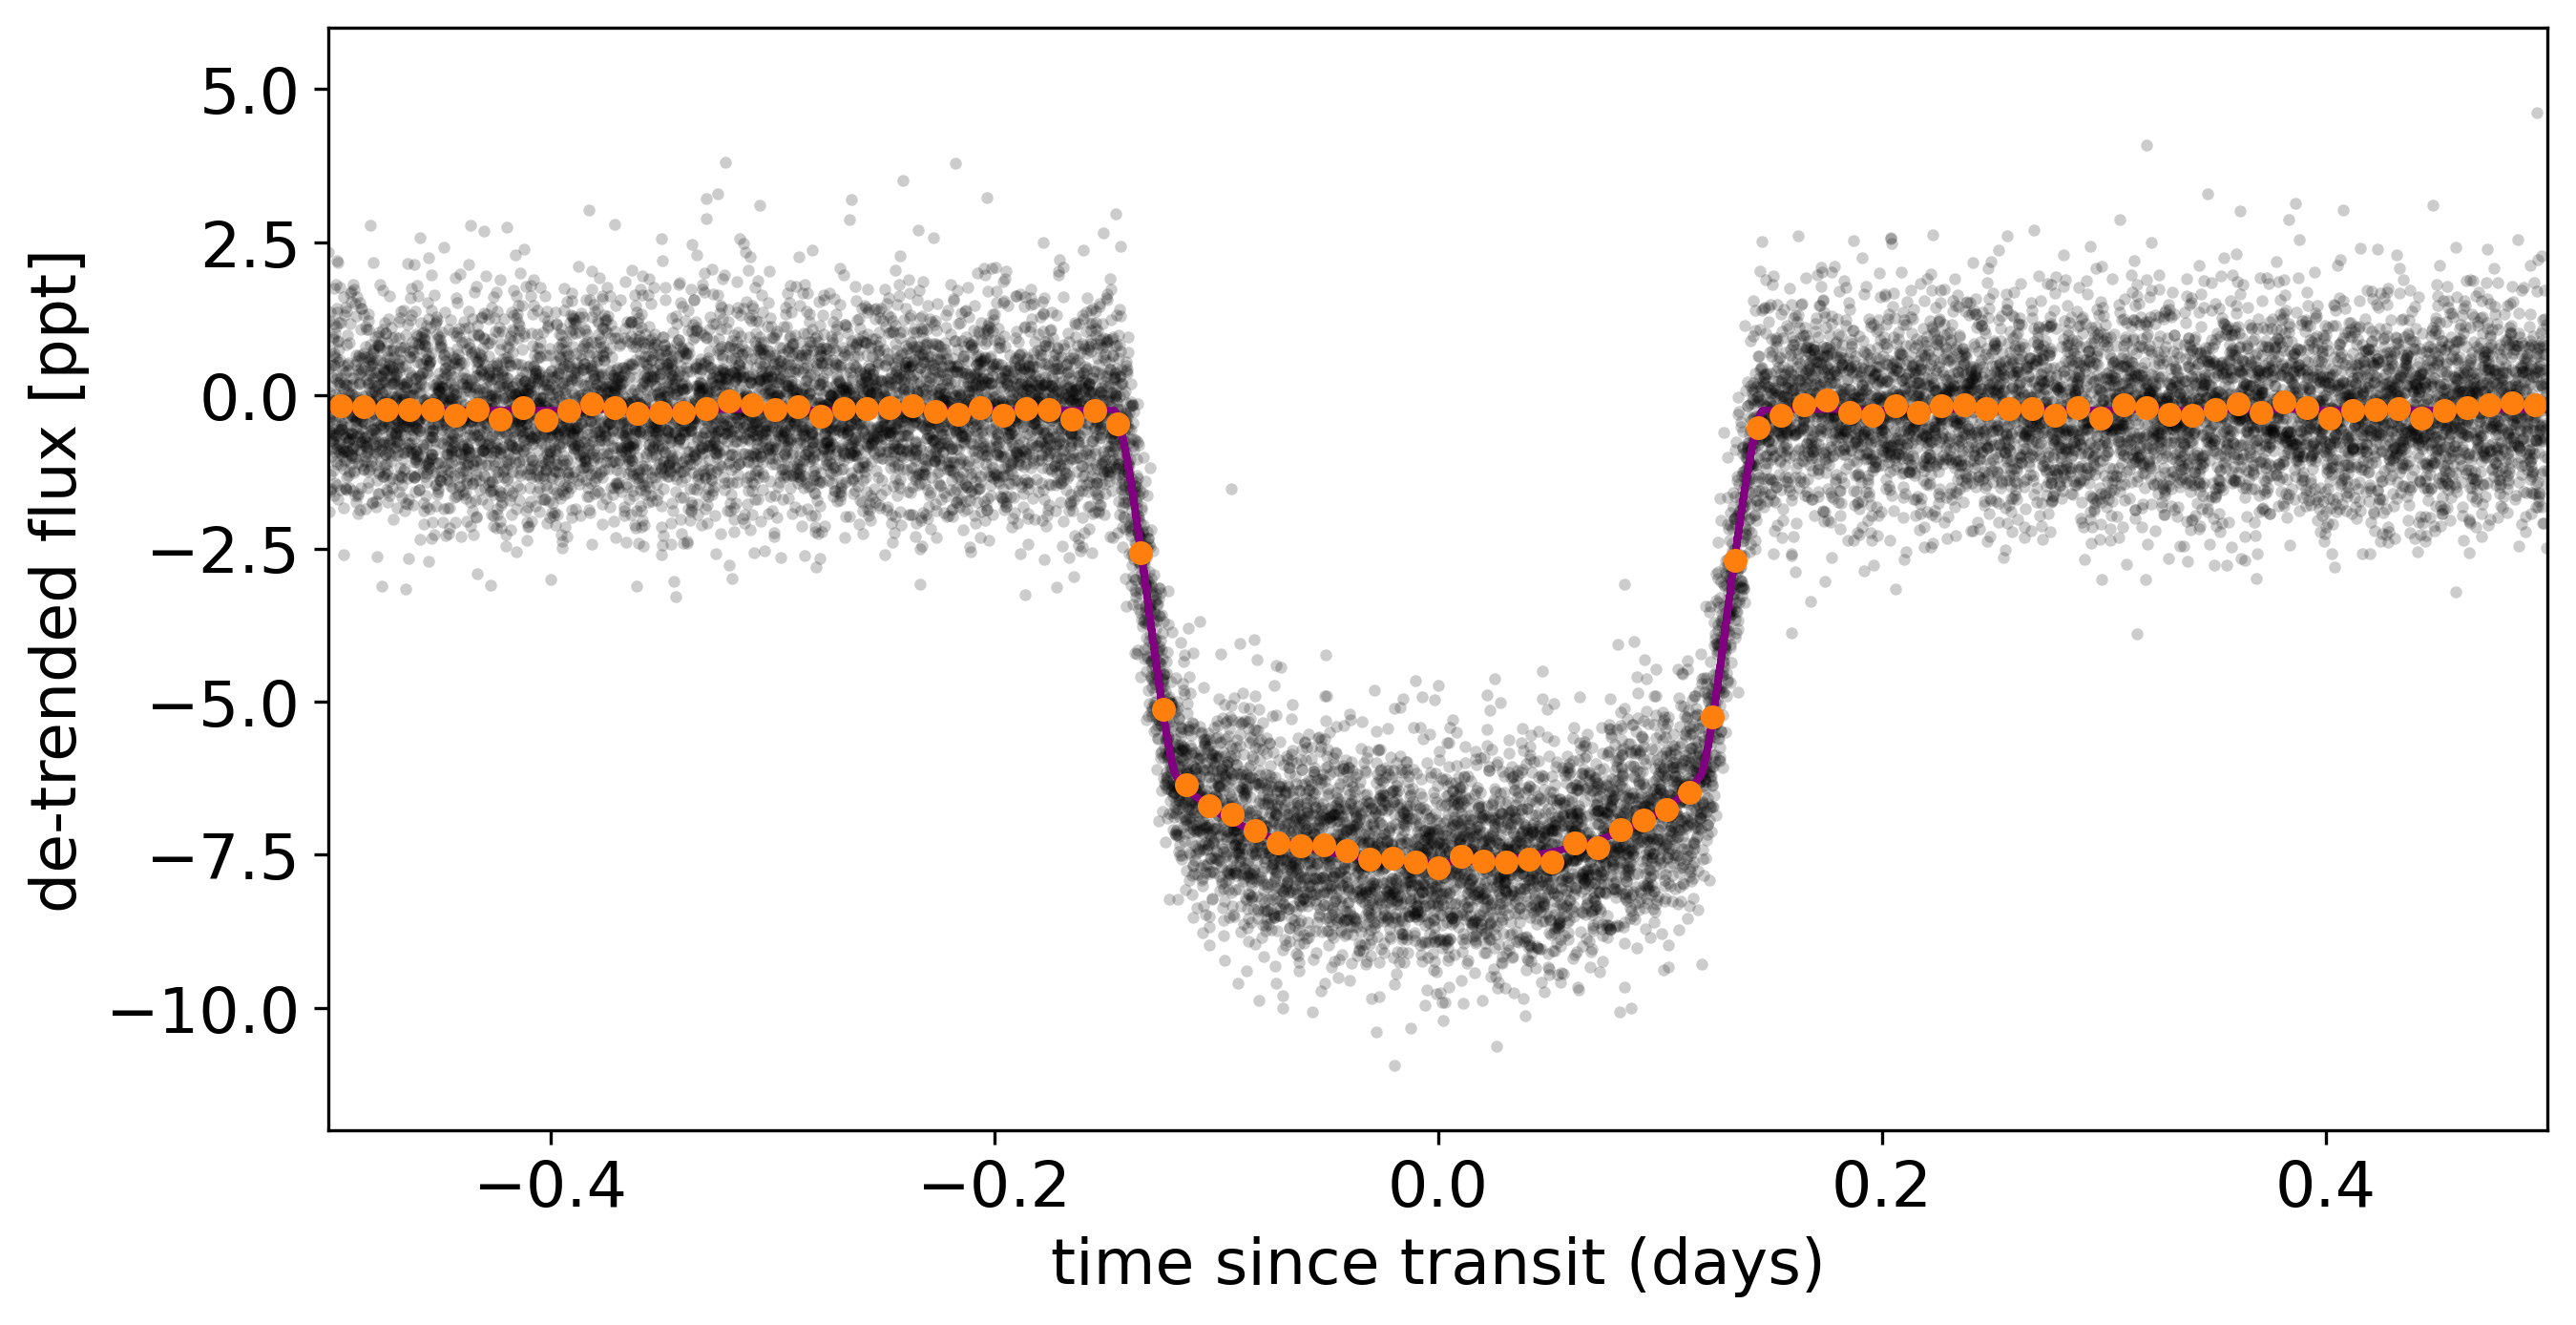
\includegraphics[width=\linewidth]{figures/best_fit_orbit.png}
    \caption{Best fit orbit overlaid on the composite TESS lightcurve.  The 1 ppt TESS precision improves upon the ground-based detection and refining the orbital properties and ephemerides.}
    \label{fig:transit}
\end{figure}


\subsubsection{Stellar rotation rate from periodogram analysis}

The TESS Sector 26 lightcurve exhibits a weak $\sim3\;$ppt peak-to-valley out-of-transit modulation on timescales comparable to the exoplanet orbit. TESS Sectors 51-53 do not show as conspicuous a modulation signal.  Figure \ref{fig:TESSmodulation} shows this modulation in the minimally processed TESS lightcurve.  During the exoplanet orbit fitting, we fit the TESS lightcurve modulation with a quasiperiodic Gaussian Process (GP) model using \texttt{celerite} \citep{celerite1,celerite2}.  The GP model fit to the entire composite lightcurve yields a period of 4.7 days; when fit to individual sectors alone the periods hover around 5.9 days.

If we attribute the TESS modulation signal to stellar activity, we obtain a rotation period $P_\mathrm{rot}$ between 4.7 and 5.9 days.  \citet{2017AJ....153..211Z} reported a $v\sin{i}=35.8\pm1.1$ km/s, or possibly as $v\sin{i}=30\pm1.1$ km/s if macroturbulence were included. We obtain a combined geometric constraint $2.85< R_\star \sin{i} (R_\odot) < 4.2 $.  The lower end of these constraints are consistent with  the 1-$\sigma$ range of $2.0 < R_\star (R_\odot) < 3.2$ provided in \citet{2017AJ....153..211Z} from different isochrones and orbit fits, and assuming a near-edge-on orbital inclination.  The Gaia \emph{DR3}-derived distance is 8\% greater than the \emph{Gaia} DR1 estimate used in \citet{2017AJ....153..211Z}; the revised larger distance would tend to increase the radius estimate by 16\% to match the observed SED in isochrone-fitting.  We would therefore expect an isochrone-deived $R_\star$ range closer to $2.5-3.14 R_\odot$, where we have dropped the 1-$\sigma$ uncertainties which had included the less certain Gaia DR 1 parallax and its uncertain correction terms.


\begin{figure}
    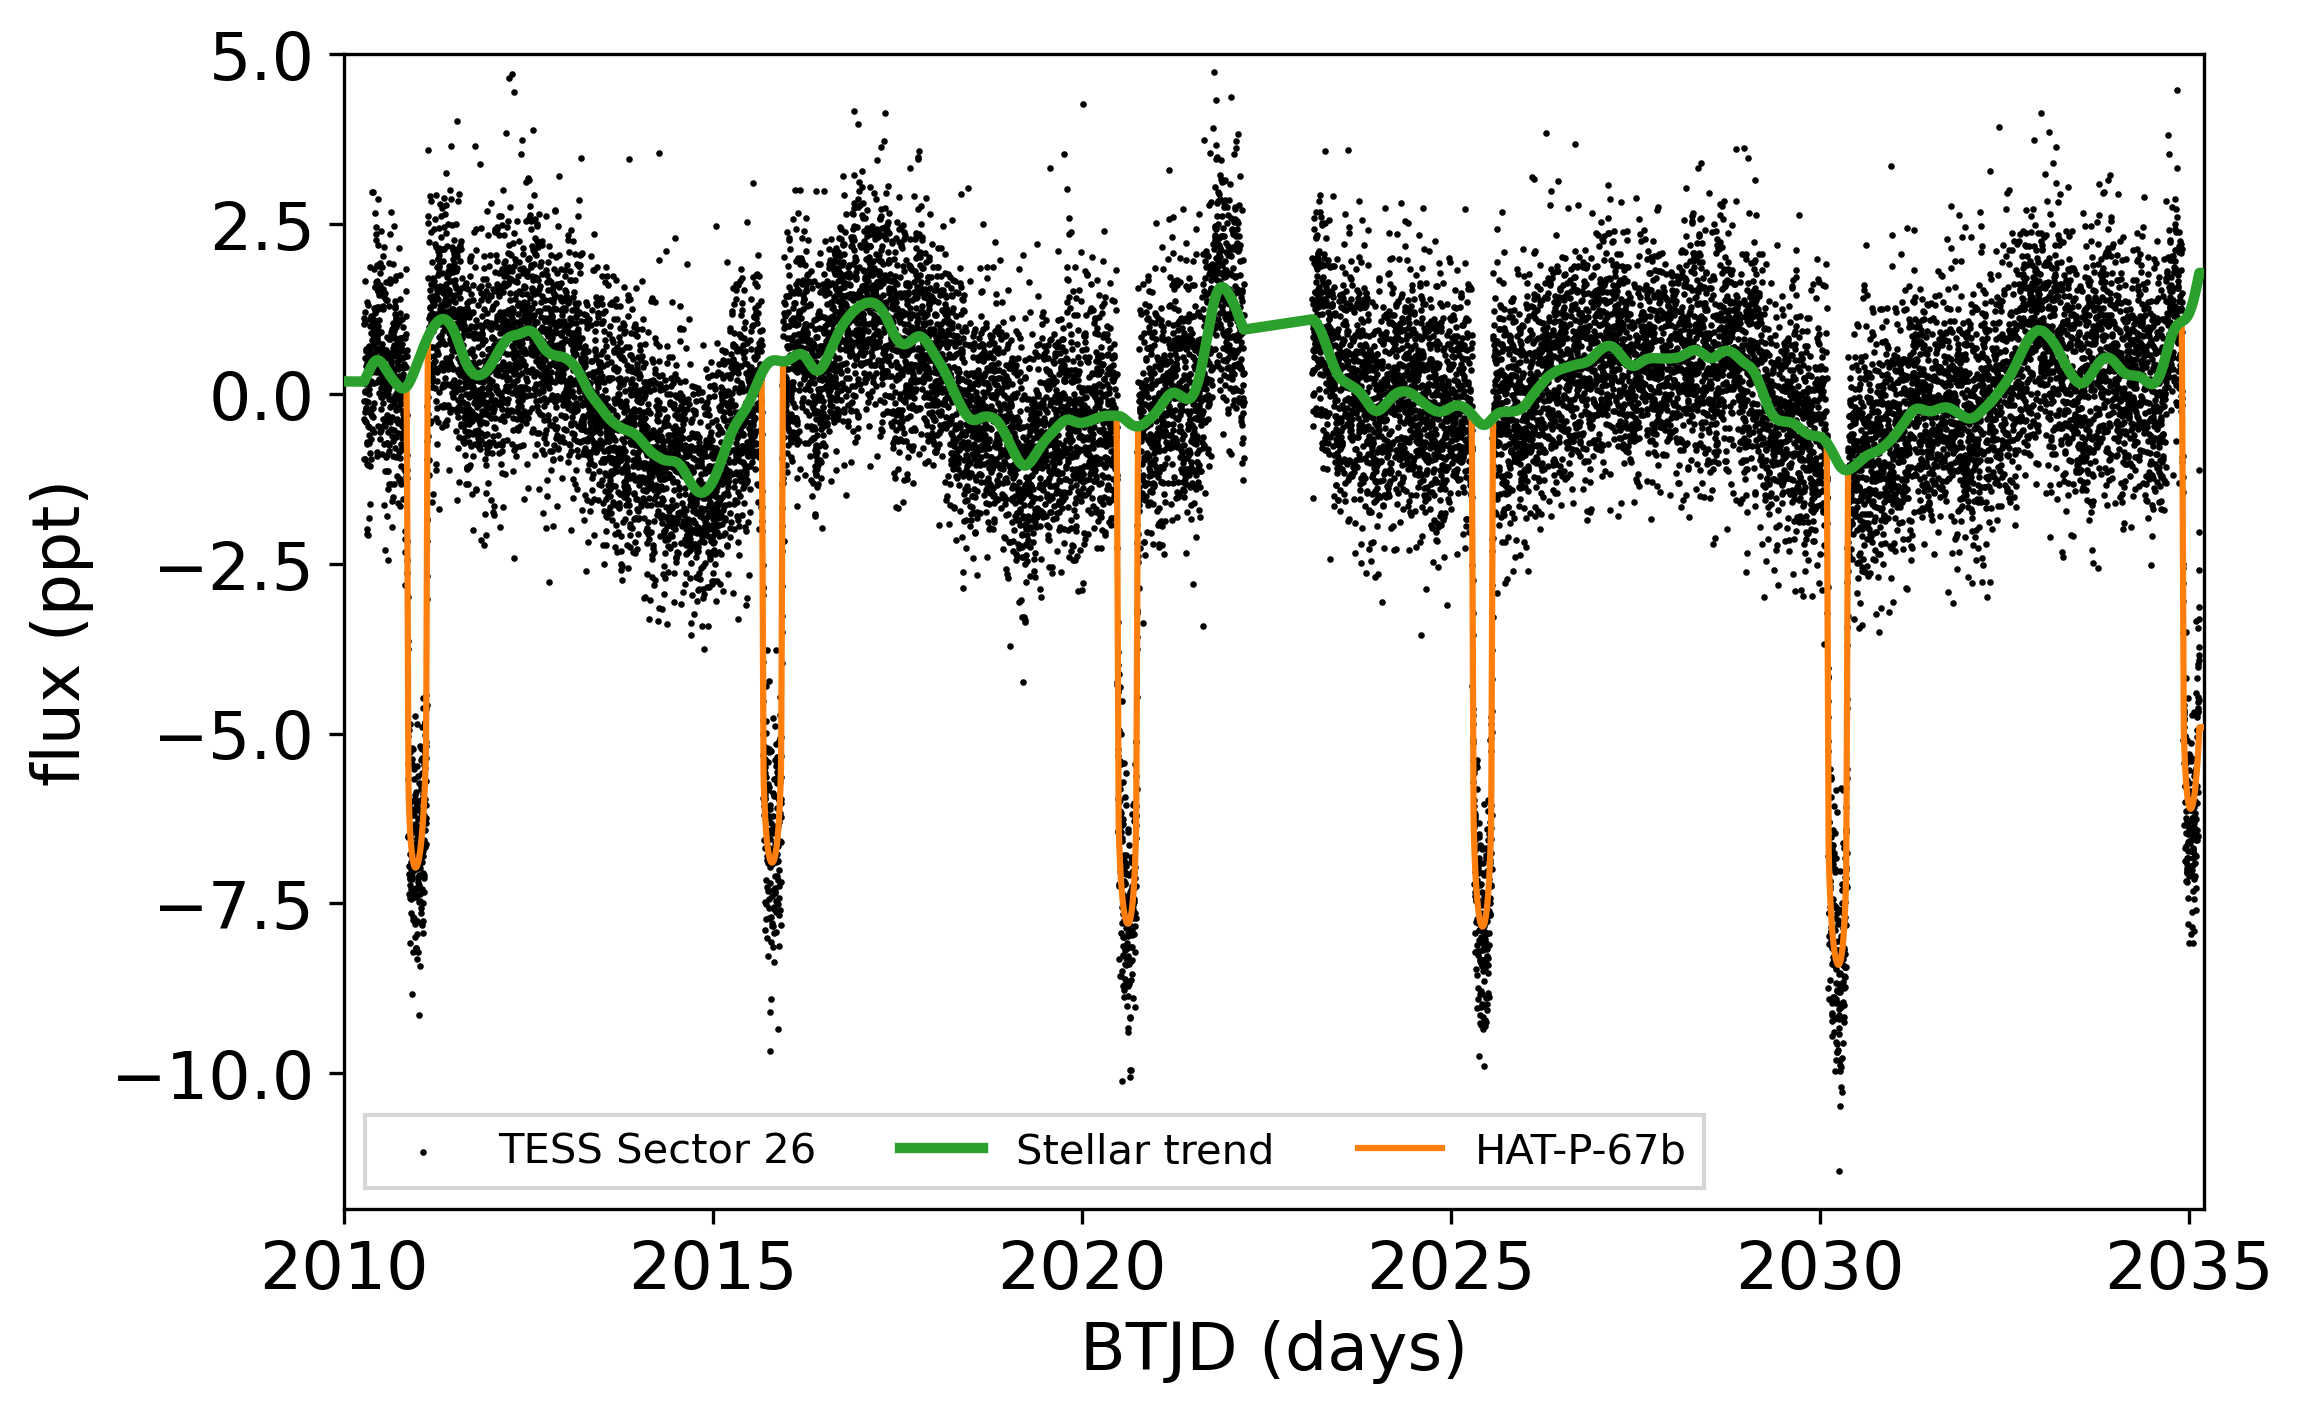
\includegraphics[width=\linewidth]{figures/TESS_S26_trend.png}
    \caption{Stellar lightcurve modulation observed in TESS Sector 26.  The stellar surface pattern speed appears to have a slightly longer period than the exoplanet orbit, causing the transit to occur earlier in the phase of the modulation upon each orbit.}
    \label{fig:TESSmodulation}
\end{figure}



\begin{deluxetable*}{lrrrh}
    \tablewidth{0pc}
    \tabletypesize{\scriptsize}
    \tablecaption{
        Revised orbital and planetary parameters
        \label{tabOrbit}
    }
    \tablehead{
        \colhead{Parameter}   &
        \colhead{Zhou et al. 2017} &
        \colhead{Ivshina \& Winn 2022} &
        \colhead{This Work} &
        \nocolhead{Alternate}
    }
    \startdata
    %%
    ~~~$P$ (days)             \dotfill    & $4.8101025_{-3.3\times 10^{-7}}^{+4.3\times 10^{-7}}$ & 4.8101046$\pm1.7\times10^{-6}$ & 4.81011 & z \\
    ~~~$T_c$ (${\rm BTJD}$)  \dotfill    & $-1038.61533_{-0.00064}^{+0.00076}$ & 1958.08059$\pm$0.00032 & 1958.07933 & z \\
    ~~~$T_{14}$ (hours)  \dotfill    & $6.9888 \pm 0.046$ &  & 7.0636 & z \\
    ~~~$T_{12} = T_{34}$ (days)  \dotfill    & $0.0229\pm0.0010$ &  &  & z \\
    ~~~$\arstar$              \dotfill    & $5.691_{-0.124}^{+0.057}$ &  &  & z \\
    ~~~$\rpl/\rstar$          \dotfill    & $0.0834\pm0.0017$ &  & 0.08231 & z \\
    ~~~$b \equiv a \cos i/\rstar$
    \dotfill    & $0.12_{-0.08}^{+0.12}$ &  & 0.45616 & z \\
    ~~~$i$ (deg)              \dotfill    & $88.8_{-1.3}^{+1.1}$ &  &  & z \\
    \enddata
\end{deluxetable*}


\subsection{HPF analysis}
Ideally we seek the pixel-to-pixel substructured spectrum of the helium exosphere, corrected for all the conceivable instrumental, telluric, and stellar contamination artifacts.  In practice, these corrections are incomplete and so some care is needed to assess the extent of contamination.  We experimented with a range of pre-processing and analysis techniques to quantify the accuracy and precision of our HPF spectra.

The raw 2D echellograms were reduced with the \texttt{Goldilocks} package\footnote{\url{https://github.com/grzeimann/Goldilocks_Documentation}}, which outputs 1D extracted spectra for the target, and two reference fibers: blank sky and a laser frequency comb (LFC).  The observations were acquired with the LFC turned off, so this unilluminated spectrum was discarded.

The sky fiber and target fiber have slightly different throughputs and illumination properties so the sky fiber must be scaled prior to subtraction from the target spectrum.  On average the target fiber sees $93\%$ of the flux of the sky reference fiber, and in detail this ratio depends on wavelength, and to-some-extent season.  We quantified the wavelength dependence by acquiring calibration observations of blank sky in both the target and sky fiber.  We applied this wavelength-based scale factor to each target spectrum's associated reference sky fiber to achieve near-imperceptible sky-line residuals.  A few lines exhibit residuals which may arise from genuine differences in the local atmospheric conditions between the target and sky fiber.

We masked spectral regions predicted to have significant telluric lines with a template generated by \texttt{telfit} \citep{2014AJ....148...53G}.  We shifted the spectral coordinates to their common barycentric-corrected reference frame \citep{2014PASP..126..838W} as implemented in \texttt{astropy} \citep{2013A&A...558A..33A,2018AJ....156..123A}.

The sky-subtraction, telluric masking, barycentric correction, and all of our other standard pre-processing steps are implemented in the open-source Python interface \texttt{muler} \citep{2022JOSS....7.4302G}.

Figure \ref{fig:HPF2022campaign} shows a zoom-in on the He 10830 region of interest.


\begin{figure}
    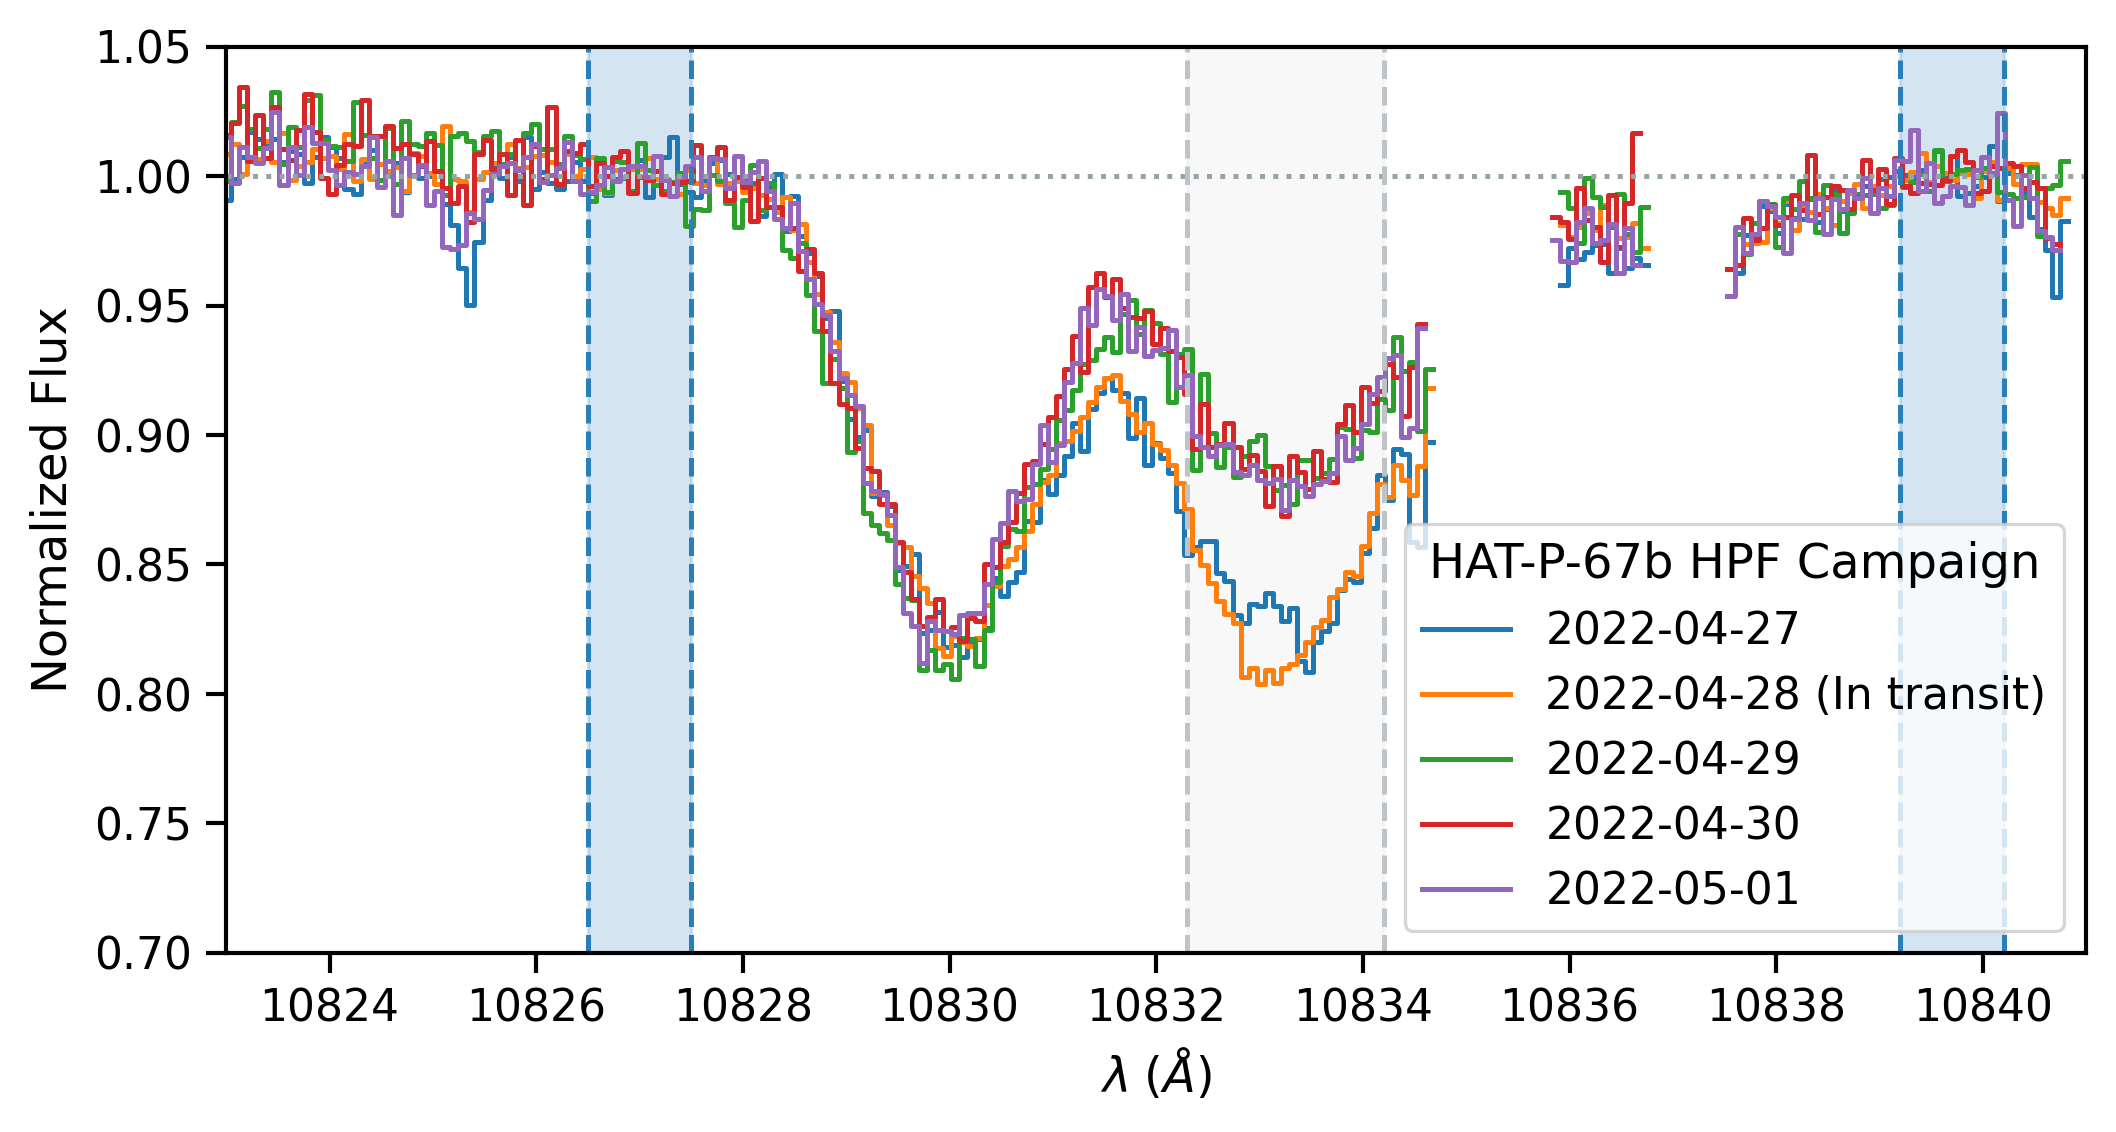
\includegraphics[width=\linewidth]{figures/HAT-P-67_2022_clean.png}
    \caption{HPF spectrum of HAT-P-67 around the spring 2022 campaign.  We see conspicuous absorption during and immediately preceding the transit, but not immediately after.  The continuum normalization indices are shown by the vertical blue shaded region and the region used for computing EW is shown in the faint gray vertical band.}
    \label{fig:HPF2022campaign}
\end{figure}


\begin{figure}
    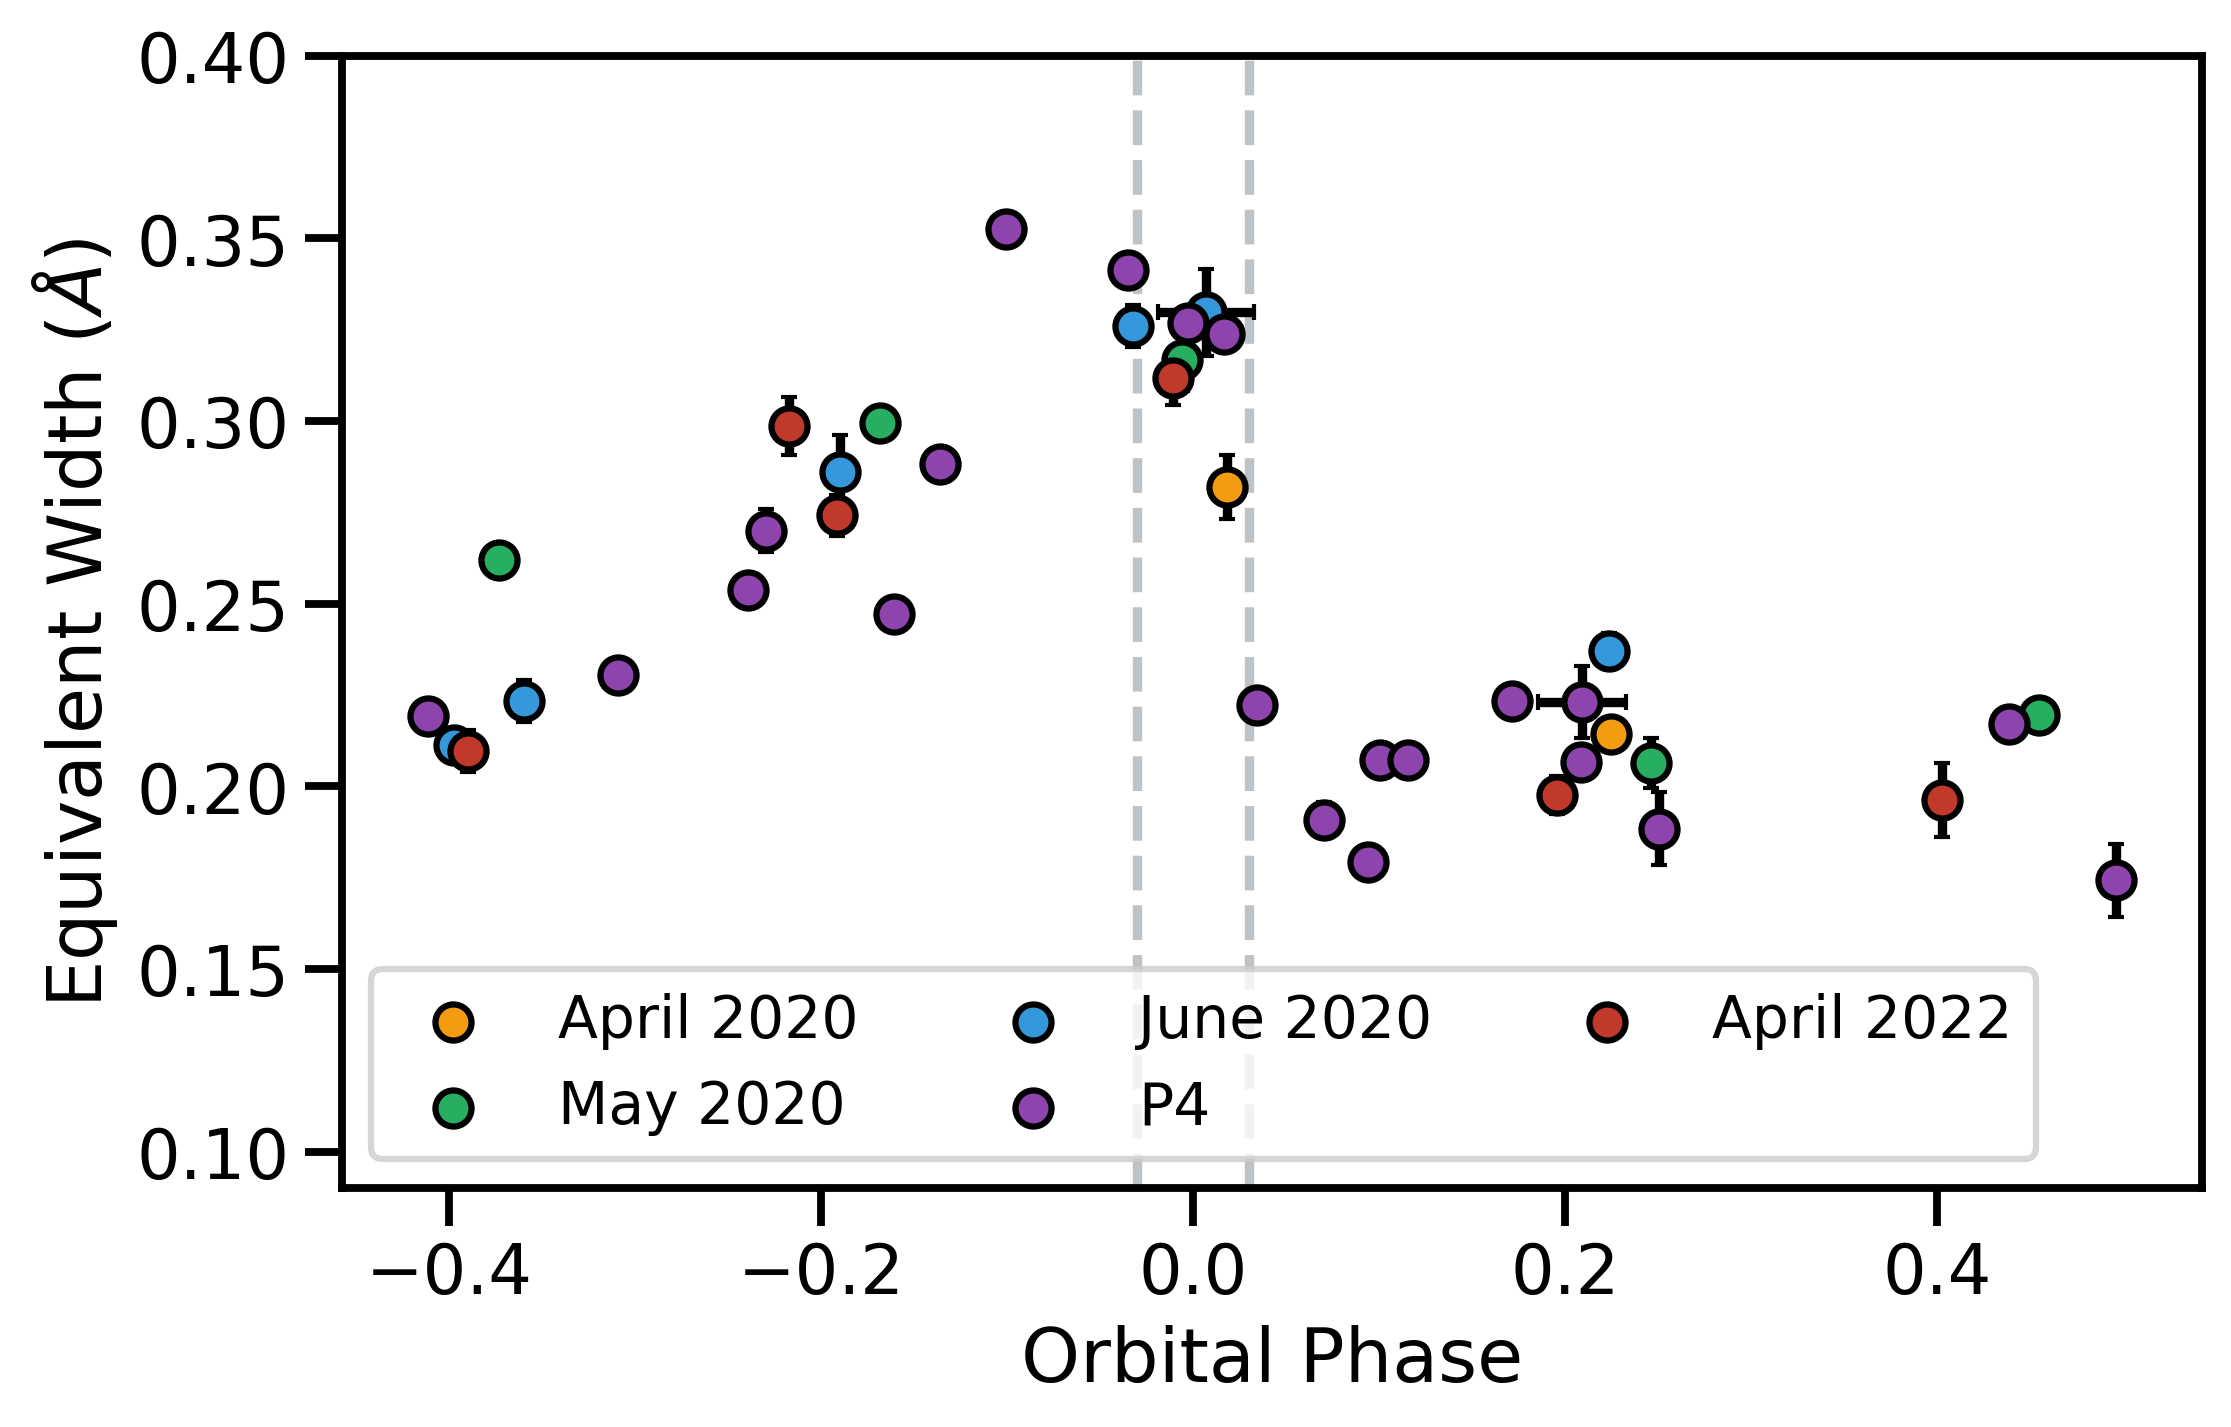
\includegraphics[width=\linewidth]{figures/HAT_P_67b_Helium10830EW_byCampaign.png}
    \caption{Time series EW lightcurve of Helium absorption in HAT-P-67b.  The system exhibits a characteristic absorption leading up to transit, followed by a sharp decline after transit passage.  }
    \label{fig:HPFtimeseries}
\end{figure}

\subsection{Calcium IR Triplet lines}

\section{Results}

\subsection{Geometry of the Escaping Exosphere}
Helium absorption occurs before the planet is in-transit, indicating a \emph{leading} tail escaping the planet. We see excess as early as 30\% of the orbital path, or about 130 planetary radii.

\subsection{Star Planet Interaction}
\subsection{Gas Motion Relative to Planet}
\subsection{Parker Winds Model}


\section{Discussion}
\subsection{Hot Spot Scenario}
The TESS 0.2\% flux variation could hypothetically arise from the foot-print of a star-planet interaction. Assuming that this increase in flux is due to a hot spot with a contrast of 200\% the ambient photosphere in the TESS bandpass, the hot spot would have a modest 5\% coverage fraction.  Thermal radiation from gravitational infall alone cannot explain the luminosity of this spot, so it would have to stem from a non-thermal cause.

\subsection{Tidal Locking Calculation}
The similarity of the rotation period with the orbital period suggests the star-planet system may be tidally locked.

\subsection{Mass Loss Rate}
A steady state mass loss rate greater than $2\times10^{12}$ g/s would erode the planet over the age of the stellar system.

\subsection{Confinement to Stellar Wind}
\subsection{Limits of Stellar Activity Metrics}
\subsection{Comparison to Other Systems}
\section{Conclusions}


\clearpage
\pagebreak


\appendix
%\section{HPF spectra post-processing}
%\label{methods-details}


\begin{acknowledgements}
    This research has made use of NASA's Astrophysics Data System.
\end{acknowledgements}

\facilities{HET (HPF), TESS, ASAS}

\software{  \texttt{pandas} \citep{mckinney10},
    \texttt{emcee} \citep{foreman13},
    \texttt{matplotlib} \citep{hunter07},
    \texttt{numpy} \citep{2020NumPy-Array},
    \texttt{scipy} \citep{2020SciPy-NMeth},
    \texttt{ipython} \citep{perez07},
    \texttt{seaborn} \citep{waskom14},
    \texttt{astropy} \citep{2022ApJ...935..167A},
    \texttt{muler} \citep{2022JOSS....7.4302G},
    \texttt{telfit} \citep{2014AJ....148...53G},
    \texttt{exoplanet} \citep{exoplanet:joss},
    \texttt{jupyter} \citep{Kluyver2016jupyter},
}


\clearpage


\bibliography{ms}

\end{document}
